% filepath: /home/dang-khoa/university/Capstone Project/Report Source/experiments/resutls.tex



\section{Kết quả và Phân tích}
Trong chương này, chúng tôi trình bày các kết quả định lượng thu được từ các thực nghiệm đã thiết lập ở phần trước. Mục tiêu là phân tích sự đánh đổi giữa độ phức tạp của việc phân hoạch không gian và tính tối ưu của quỹ đạo đầu ra. Toàn bộ các thực nghiệm được thực hiện trên máy tính cá nhân với cấu hình: CPU AMD Ryzen 7 4800H 2.9 GHz, RAM 16GB, hệ điều hành Ubuntu 24.04.
\subsection{Phân tích Môi trường 2D đơn giản: Tác động của Phân hoạch lồi}

% grid 4 images
\begin{figure}[!htp]
    \centering
    \begin{subfigure}[b]{0.48\textwidth}
        \centering
        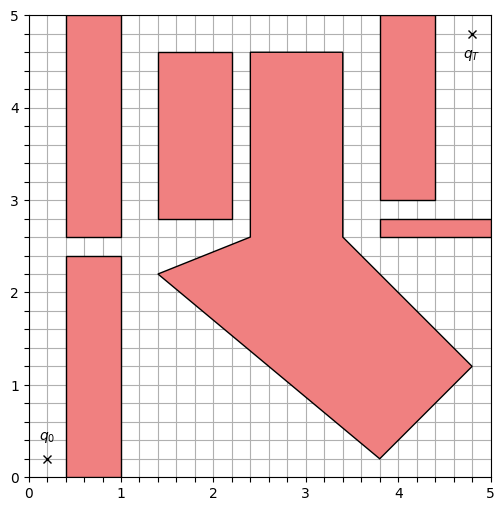
\includegraphics[width=\textwidth]{experiments/image/2d-env.png}
        \caption{Không gian 2D với vật cản (vùng màu đỏ) ban đầu}
        \label{fig:result_a}
    \end{subfigure}
    \hfill
    \begin{subfigure}[b]{0.48\textwidth}
        \centering
        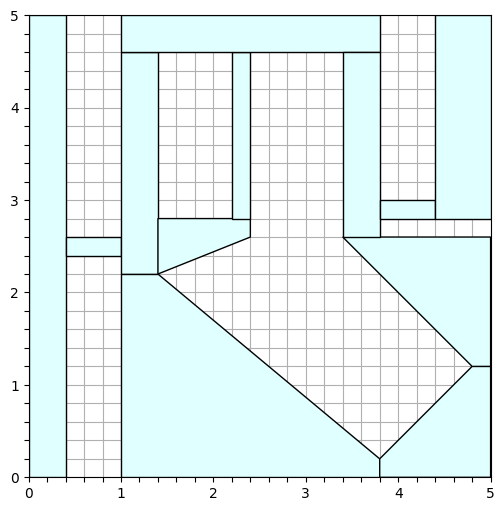
\includegraphics[width=\textwidth]{experiments/image/manual_decompose.png}
        \caption{Kết quả Phân hoạch thủ công}
        \label{fig:result_b}
    \end{subfigure}
    
    \vspace{0.5cm}
    
    \begin{subfigure}[b]{0.48\textwidth}
        \centering
        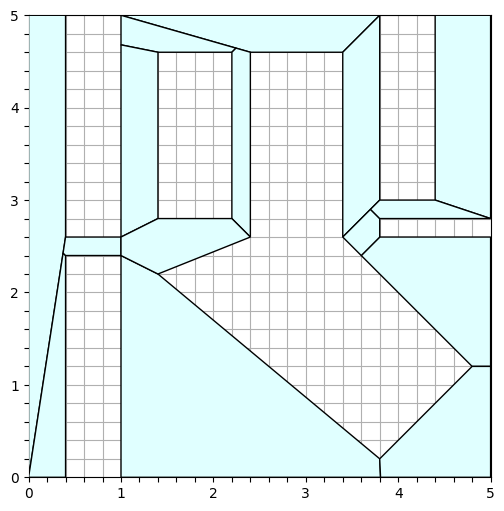
\includegraphics[width=\textwidth]{experiments/image/ACD_decompose.png}
        \caption{Kết quả Phân hoạch ACD}
        \label{fig:result_c}
    \end{subfigure}
    \hfill
    \begin{subfigure}[b]{0.48\textwidth}
        \centering
        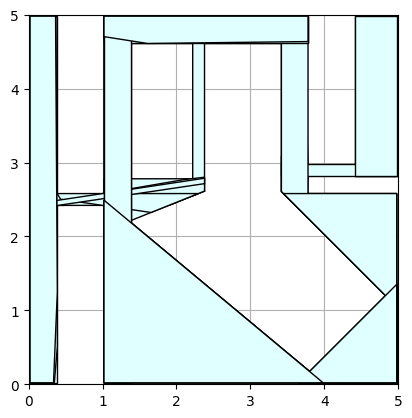
\includegraphics[width=\textwidth]{experiments/image/VCC_decompose.png}
        \caption{Kết quả Phân hoạch VCC}
        \label{fig:result_d}
    \end{subfigure}
    
    \caption[So sánh các phương pháp phân hoạch]{So sánh chất lượng các vùng lồi được phân hoạch bởi các giải thuật khác nhau. Số lượng tập lồi tăng dần từ (b) đến (d), cho thấy sự cải thiện về độ chính xác nhưng tăng độ phức tạp tính toán.}
    \label{fig:results_grid}
\end{figure}


Kết quả thực nghiệm đối với các giải thuật phân hoạch tự động cho thấy sự tương phản rõ rệt về chiến lược biểu diễn không gian cấu hình cũng như chi phí tính toán
giữa hai phương pháp tiếp cận chủ đạo là ACD và VCC. Đối với giải thuật Phân hoạch Lồi Xấp xỉ (ACD), 
kết quả đạt được thể hiện như hình \ref{fig:result_c} ưu thế vượt trội trong môi trường hình học 2D khi chỉ tạo ra 15 vùng lồi, một con số tiệm cận sát với mức tối ưu của phương pháp phân hoạch thủ công là 12 vùng. 
Hiệu suất này được củng cố bởi thời gian xử lý nhanh, chỉ xấp xỉ 0,01 giây, hoàn toàn phù hợp với độ phức tạp lý thuyết $O(nr^2)$ \cite{LienAmato2006} của thuật toán khi xử lý các đa giác có số lượng đỉnh lõm không quá lớn. 
Việc ACD có khả năng kiểm soát mức độ chi tiết thông qua tham số lõm $\tau$ cho phép hệ thống duy trì được sự cân bằng giữa độ chính xác hình học và số lượng vùng lồi tối giản, từ đó giảm thiểu số lượng biến nhị phân trong bài toán quy hoạch nguyên-hỗn hợp (MICP) 
của GCS framework. \\
Ngược lại, giải thuật Visibility VCC (VCC) lại mang đến một cấu trúc phân hoạch dày đặc và phức tạp hơn với số lượng vùng lồi dao động từ 33 đến 35 vùng. Sự thiếu ổn định về số lượng vùng phân hoạch giữa các lần thực thi xuất phát trực tiếp 
từ tính chất ngẫu nhiên của bước lấy mẫu $n$ điểm trong không gian cấu hình tự do $C_{free}$ để xây dựng đồ thị khả kiến đã được nêu ở phần \ref{VCC}. Mặc dù sự chênh lệch khoảng 1-3 vùng lồi tại các khu vực hành lang hẹp là mức sai số có thể chấp nhận được, nhưng tổng số lượng vùng lồi lớn đã tạo 
ra một gánh nặng tính toán đáng kể cho bộ giải Mosek do số lượng biến nhị phân $y_e$ tăng lên theo tỉ lệ xấp xỉ $2|I|$. Thời gian hội tụ của VCC trong môi trường 2D thực tế không mang lại hiệu quả cao cho các ứng dụng yêu cầu phản hồi tức thời so với các kỹ thuật phân hoạch 
đa giác trực tiếp như ACD. Tuy nhiên, cần phải nhìn nhận rằng VCC được thiết kế như một phương pháp lai ghép mạnh mẽ để xử lý các không gian cấu hình cao chiều, nơi các vật cản không được xác định tường minh bằng các đa giác mà thông qua các bộ kiểm tra va chạm chung. 
Trong các hệ thống có số chiều lớn như cánh tay robot 7 bậc tự do (7-DoF), việc lấy mẫu và tìm lớp phủ clique giúp VCC tự động hóa quá trình đặt các điểm mầm chiến lược cho thuật toán IRIS, điều mà các phương pháp phân hoạch hình học 2D đơn giản không thể thực hiện được. 
Do đó, việc áp dụng VCC vào môi trường 2D trong thực nghiệm này chủ yếu đóng vai trò kiểm chứng khả năng bao phủ toàn cục và tính an toàn của quỹ đạo.

% filepath: /home/dang-khoa/university/Capstone Project/Report Source/experiments/resutls.tex

% Grid 3 ảnh (2 ảnh trên, 1 ảnh dưới giữa)
\begin{figure}[!htp]
    \centering
    \begin{subfigure}[b]{0.48\textwidth}
        \centering
        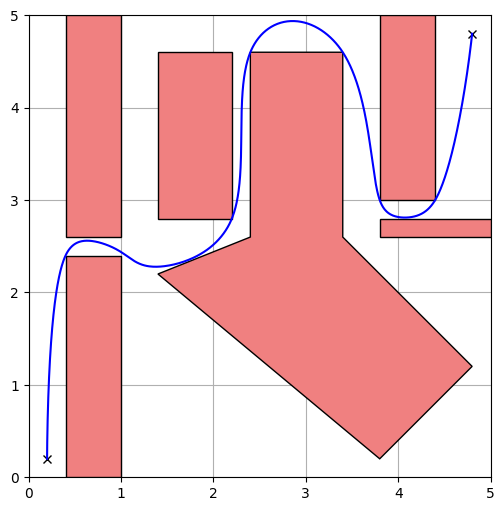
\includegraphics[width=\textwidth]{experiments/image/manual_traj.png}
        \caption{Qũy đạo chuyển động với phân hoạch thủ công}
        \label{fig:result_manual}
    \end{subfigure}
    \hfill
    \begin{subfigure}[b]{0.48\textwidth}
        \centering
        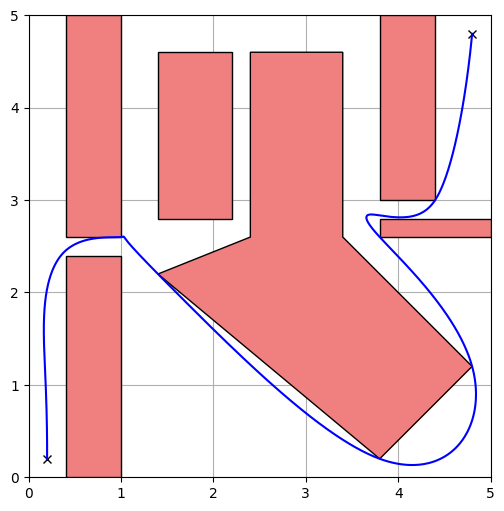
\includegraphics[width=\textwidth]{experiments/image/ACD_traj.png}
        \caption{Qũy đạo chuyển động với phân hoạch ACD}
        \label{fig:result_acd}
    \end{subfigure}
    
    \vspace{0.5cm}
    
    \begin{subfigure}[b]{0.48\textwidth}
        \centering
        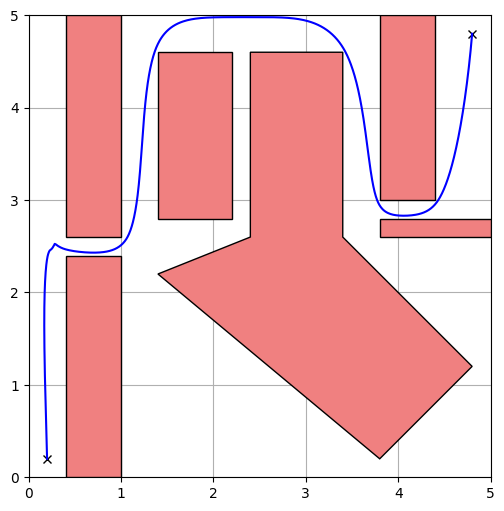
\includegraphics[width=\textwidth]{experiments/image/VCC_traj.png}
        \caption{Qũy đạo chuyển động với phân hoạch VCC}
        \label{fig:result_vcc}
    \end{subfigure}
    
    \caption[So sánh các quỹ đạo chuyển động cho từng phương pháp phân hoạch]{So sánh chất lượng các quỹ đạo được hoạch định cho tập các vùng lồi được tạo bởi các giải thuật ở trên.}
    \label{fig:results_grid_3}
\end{figure}


\begin{table}[htbp]
\centering
\caption{So sánh hiệu năng giữa các phương pháp lập kế hoạch quỹ đạo}
\label{tab:comparison_all}
\resizebox{\textwidth}{!}{%
\begin{tabular}{lcccccc}
\toprule
\textbf{Phương pháp} 
& \textbf{Thời gian phân hoạch (s)} 
& \textbf{Số vùng} 
& \textbf{Thời gian giải (s)} 
& \textbf{Time cost (s)} 
& \textbf{Path cost (rounded)} 
& \textbf{Tổng thời gian (s)} \\
\midrule
VCC       
& 5.7807 
& 33 
& 269.9363 
& 13.2217 
& 24.4365 
& 275.7170 \\
ACD             
& 0.0109 
& 15 
& 4.3105   
& 12.7875 
& 24.6286 
& 4.3214 \\
Phân hoạch thủ công 
& --     
& 12 
& 3.9005   
& 13.3565 
& 27.8805 
& 3.9005 \\
\bottomrule
\end{tabular}}
\end{table}



Sau khi hoàn tất giai đoạn phân hoạch không gian tự do thành các tập hợp vùng lồi, chúng tôi tiến hành thực hiện bài toán hoạch định quỹ đạo dựa trên khung làm việc Đồ thị các Tập lồi (Graphs of Convex Sets - GCS). Mục tiêu của giai đoạn này là tìm kiếm một lộ trình tối ưu không chỉ về mặt hình học mà còn phải đáp ứng các ràng buộc về động lực học và độ trơn của quỹ đạo. Để đạt được sự cân bằng giữa thời gian thực thi vật lý ($T_{duration}$) và nỗ lực điều khiển (Control effort), hàm mục tiêu tổng hợp (Rounded Cost) được thiết lập như sau:
$$Rounded Cost \approx (1 \times T_{duration}) + \sum \left( 0.1 \times \int_{0}^{T_e} \|\text{a}(t)\|^2 dt \right)$$

Trong đó, trọng số cho thời gian thực thi được đặt là $w_{t}=1$ và hệ số điều chuẩn đạo hàm bậc hai (gia tốc) là $\epsilon = 0.1$ nhằm giảm thiểu hiện tượng rung động (jerk) khi robot di chuyển qua các ranh giới vùng lồi. Các kết quả định lượng về hiệu suất tính toán và chất lượng quỹ đạo được phân tích chi tiết dựa trên dữ liệu thu được từ bộ giải Mosek.

\subsubsection{Hiệu suất tính toán và Khả năng đáp ứng thời gian thực}

Kết quả thực nghiệm cho thấy một sự tương quan phi tuyến tính chặt chẽ giữa số lượng vùng lồi được phân hoạch và thời gian hội tụ của bộ giải. Phương pháp \textbf{VCC} cho thấy hiệu năng kém nhất trong môi trường thực nghiệm 2D. Mặc dù số lượng vùng lồi được tạo ra (33 vùng) chỉ cao hơn gấp đôi so với ACD, nhưng thời gian giải bài toán tối ưu hóa lại rất lớn lên tới xấp xỉ 269,94 giây. Hiện tượng này xuất phát từ việc gia tăng số lượng vùng lồi dẫn đến sự bùng nổ của các biến quyết định nhị phân  và các ràng buộc nón phối cảnh liên kết, khiến không gian tìm kiếm tổ hợp vượt quá khả năng xử lý hiệu quả của bộ giải trong thời gian thực.

Ngược lại, phương pháp \textbf{ACD} thể hiện tính thực tiễn vượt trội khi tổng thời gian thực thi (bao gồm cả phân hoạch và giải quỹ đạo) chỉ mất 4,32 giây, nhanh gấp khoảng 64 lần so với VCC. Kết quả này khẳng định rằng đối với các ứng dụng di động trong môi trường 2D, một cấu trúc phân hoạch tối giản (15 vùng) là yếu tố tiên quyết để duy trì khả năng phản hồi nhanh của hệ thống. Trong khi đó, phương pháp \textbf{Phân hoạch thủ công} mặc dù đạt thời gian giải nhanh nhất (3,90 giây) do cấu trúc đồ thị đơn giản (12 vùng), nhưng không được xem là giải pháp khả thi cho các hệ thống tự hành do đòi hỏi sự can thiệp trực tiếp từ con người, vốn là một rào cản lớn đối với tính tự chủ của robot.

\subsubsection{Chất lượng Quỹ đạo và Sự đánh đổi giữa các Mục tiêu Tối ưu}

Chất lượng của quỹ đạo được đánh giá thông qua sự đánh đổi giữa thời gian di chuyển thực tế và giá trị tối ưu của hàm mục tiêu (Path cost).

\begin{itemize}
\item \textbf{Phương pháp VCC}: Đạt giá trị Path cost thấp nhất ($24,44$), đại diện cho nghiệm tối ưu nhất về mặt toán học. Việc chia nhỏ không gian thành nhiều vùng lồi diện tích nhỏ cho phép bộ giải có nhiều "không gian tự do" hơn để tinh chỉnh đường cong Bézier, từ đó tối ưu hóa nỗ lực điều khiển và giảm thiểu tối đa các pha phạt gia tốc. Tuy nhiên, thời gian thực thi vật lý ($13,22$ giây) lại chậm hơn ACD, cho thấy hệ thống chấp nhận di chuyển với vận tốc thấp hơn để đổi lấy độ trơn tuyệt đối. 
\item \textbf{Phương pháp ACD}: Mang lại kết quả thực dụng nhất khi robot hoàn thành nhiệm vụ với thời gian ngắn nhất ($12,79$ giây). Mặc dù Path cost ($24,63$) cao hơn nhẹ so với VCC, nhưng sự chênh lệch này không đáng kể trong vận hành thực tế. Điều này chứng tỏ ACD đã tạo ra một quỹ đạo "thực dụng": chạy nhanh, đủ mượt mà và duy trì được tính toán hiệu quả. 
\item \textbf{Phân hoạch thủ công}: Thể hiện hiệu năng kém nhất về mặt chất lượng quỹ đạo với Path cost cao nhất ($27,88$) và thời gian di chuyển lâu nhất ($13,36$ giây). Nguyên nhân chủ yếu nằm ở việc phân chia vùng dựa trên trực giác con người thường tạo ra các vùng lồi thô, các vùng có thể to nhưng hình dạng không tối ưu cho robot lách qua, hoặc các điểm nối giữa các vùng bị đặt ở vị trí xấu, khiến robot phải đi đường vòng hoặc phanh gấp tại các giao điểm.
\end{itemize}

Tóm lại, thông qua các chỉ số đo lường thực nghiệm, chúng tôi xác định \textbf{ACD} là giải pháp tối ưu cho các bài toán hoạch định quỹ đạo 2D, đảm bảo được sự cân bằng giữa chi phí tính toán và hiệu suất vận hành thực tế. Trong khi đó, phương pháp VCC dù cho thấy tiềm năng về tính tối ưu toán học nhưng lại gặp rào cản lớn về thời gian giải, khiến nó phù hợp hơn cho các ứng dụng ngoại tuyến hoặc trong các không gian cấu hình cao chiều phức tạp.

\subsection{Phân tích Thực nghiệm trên Môi trường Mê cung Phức tạp}

Trong phần thực nghiệm này, chúng tôi mở rộng quy mô kiểm chứng sang môi trường mê cung có độ phức tạp tổ hợp lớn nhằm đánh giá khả năng của khung làm việc GCS trong việc kết hợp hài hòa giữa tối ưu hóa rời rạc và liên tục. Để đảm bảo tính khách quan và độ tin cậy về mặt thống kê, các thực nghiệm được thực hiện trên 10 cấu trúc mê cung khác nhau, được sinh ngẫu nhiên bằng thuật toán DFS với kích thước $25 \times 25 = 625$ ô. Trong mỗi mê cung, chúng tôi loại bỏ ngẫu nhiên 100 bức tường để tạo ra các lộ trình đa dạng, buộc bộ lập kế hoạch phải tìm kiếm nghiệm tối ưu trên một đồ thị có cấu trúc liên thông phức tạp.

Các tham số tối ưu hóa được thiết lập đồng nhất cho tất cả các mẫu thử nghiệm với đường cong Bézier bậc $d = 6$, đảm bảo độ trơn liên tục cấp $C^2$. Hàm mục tiêu tập trung tối thiểu hóa thời gian thực thi kết hợp với điều chuẩn đạo hàm bậc hai ($\epsilon = 10^{-1}$) nhằm phạt các gia tốc quá lớn. Bộ giải \textit{Mosek} được sử dụng để xử lý bài toán SOCP thu được từ kỹ thuật nới lỏng lồi.

\begin{figure}[!htp]
    \centering
    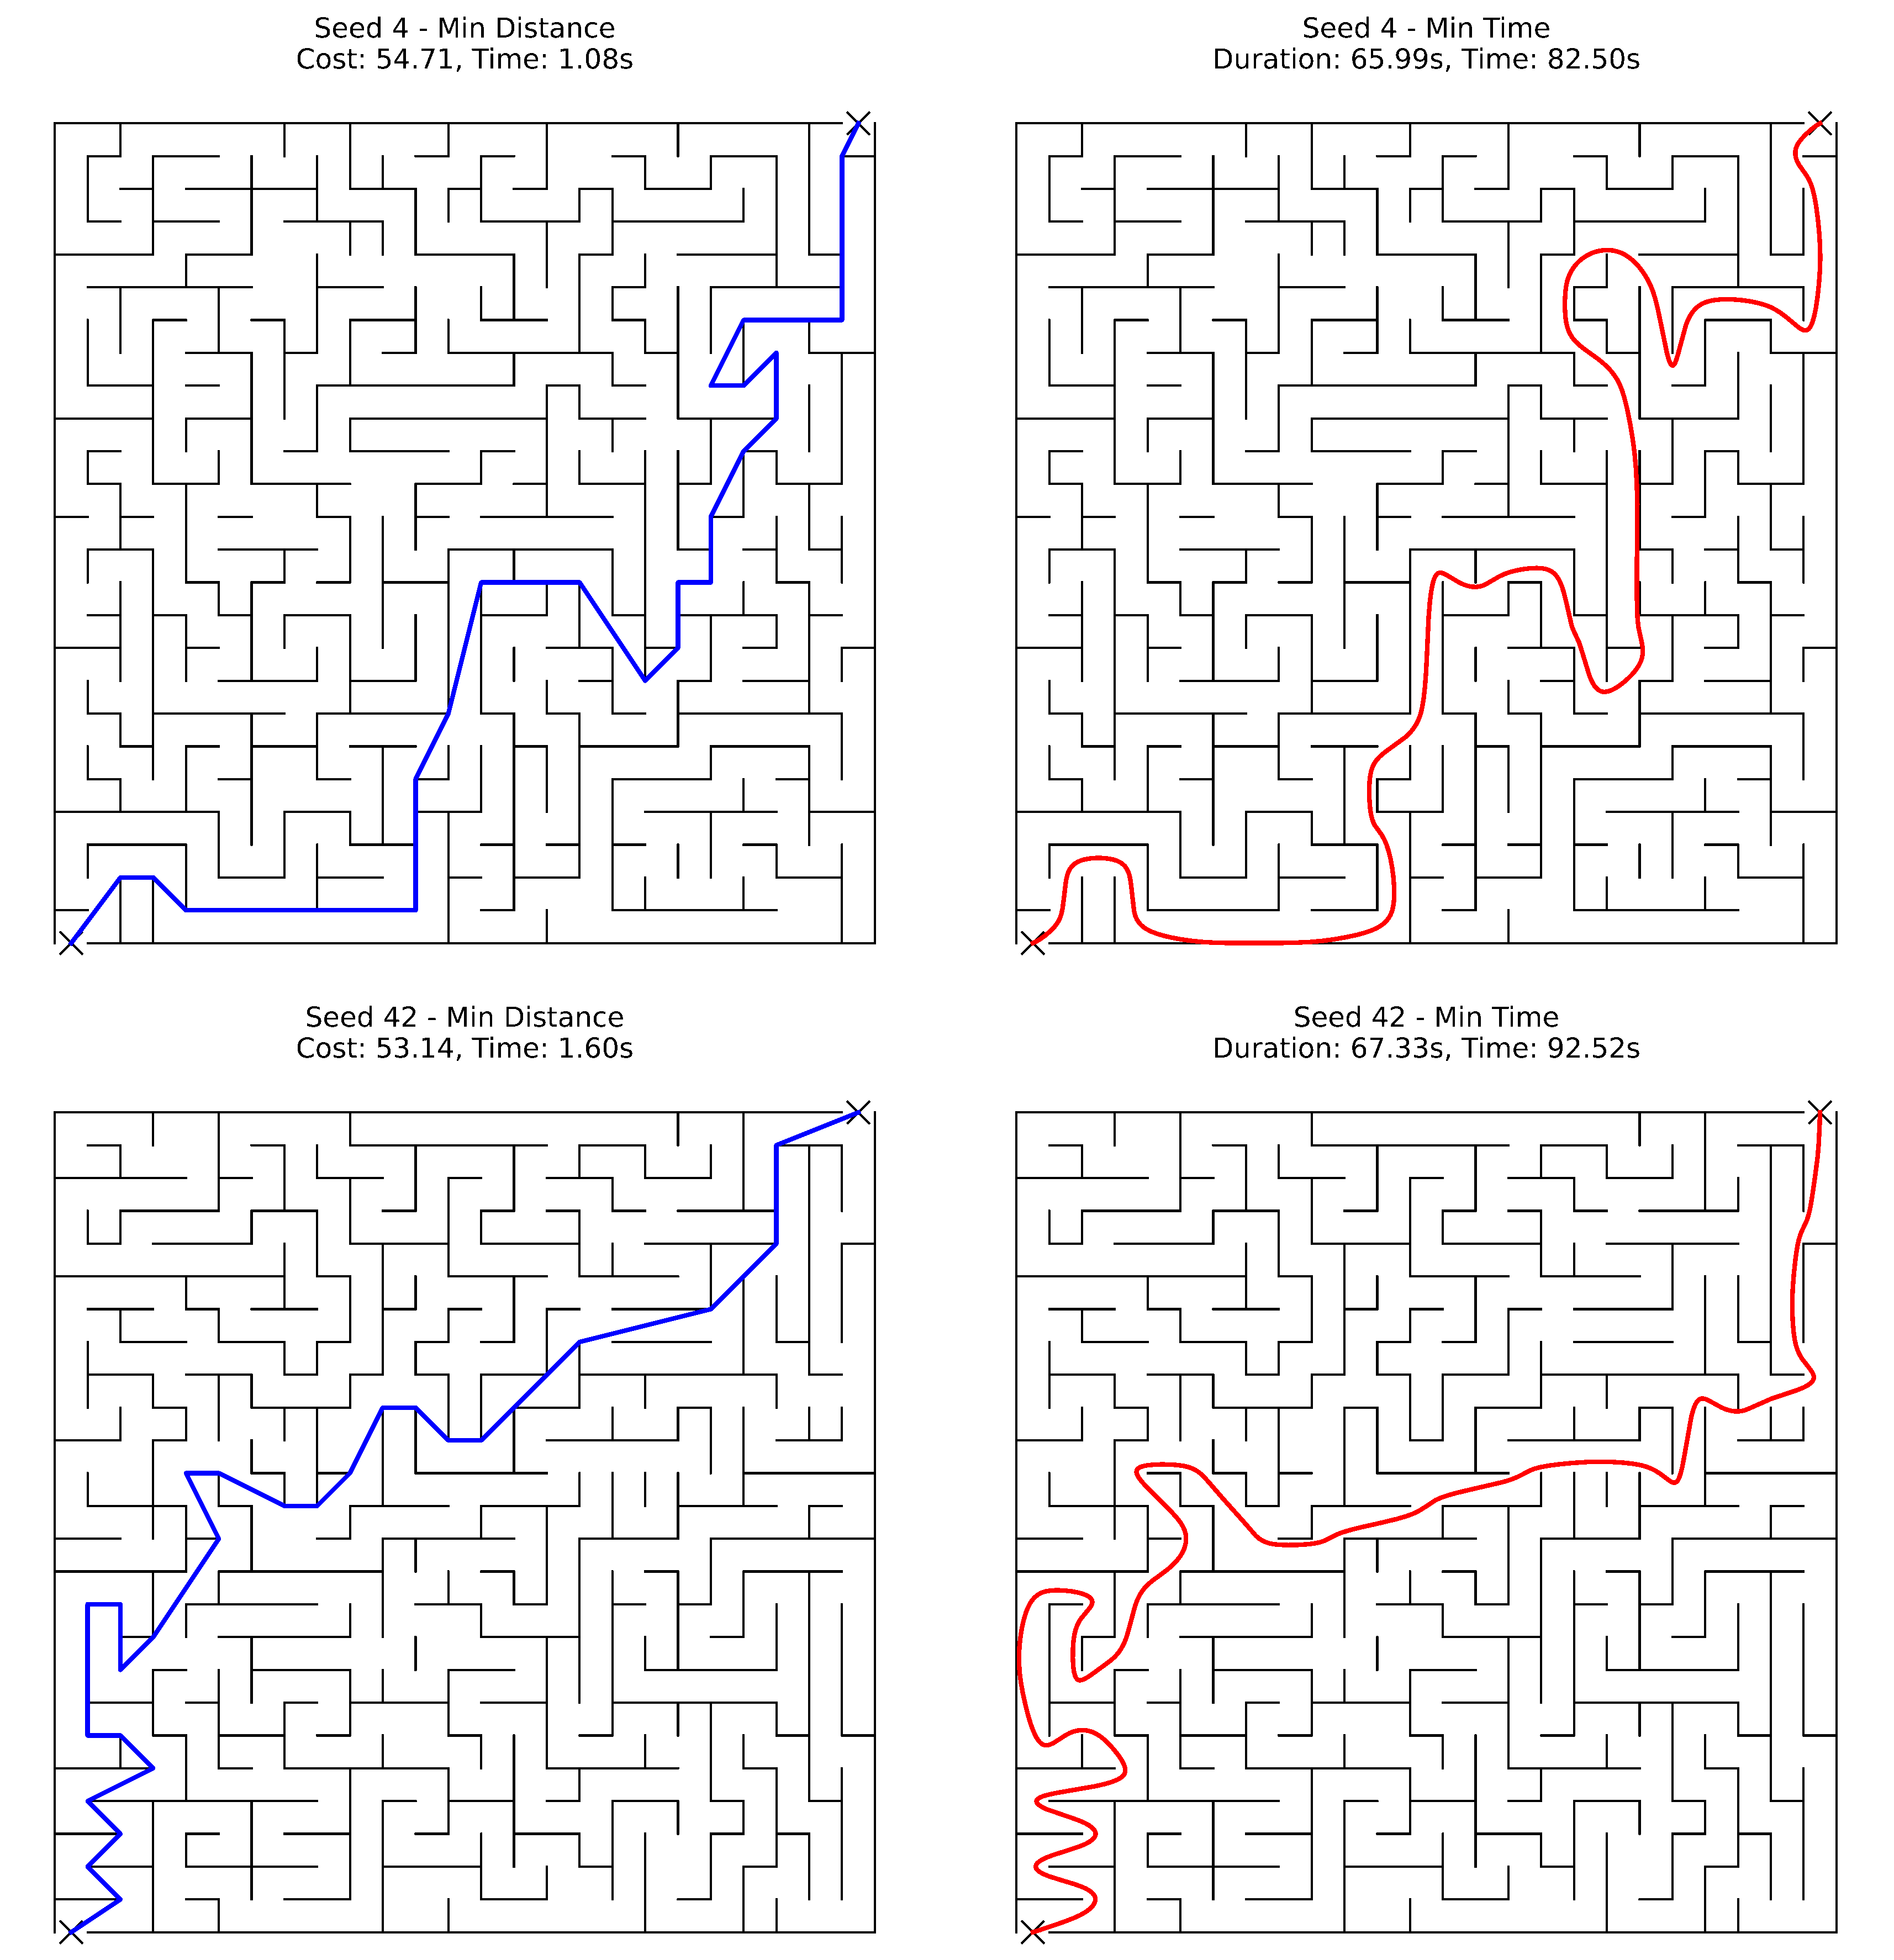
\includegraphics[width=0.7\textwidth]{experiments/image/maze-1.png}
    \caption{Quỹ đạo chuyển động cho 1 số mê cung}
    \label{fig:maze_results}
\end{figure}

\subsubsection{Phân tích Hiệu suất Tính toán và Chi phí Tối ưu}

Dựa trên dữ liệu thu thập từ 10 mẫu thử nghiệm, chúng tôi tiến hành so sánh đối chiếu giữa hai phương pháp:
\begin{itemize}
    \item \textbf{Linear GCS}: tối thiểu hóa độ dài hình học.
    \item \textbf{Bezier GCS}: tối thiểu hóa thời gian với ràng buộc động lực học.
\end{itemize}

\begin{table}[!ht]
    \centering
    \caption{Thống kê kết quả thực nghiệm trên 10 mẫu mê cung ngẫu nhiên}
    \begin{tabular}{|l|c|c|c|}
        \hline
        \textbf{Chỉ số (Metric)} 
        & \textbf{Linear GCS} 
        & \textbf{Bezier GCS} 
        & \textbf{Đơn vị} \\
        \hline
        Thời gian giải trung bình (Mean) 
        & 1,28 
        & 85,22 
        & s \\
        \hline
        Thời gian giải trung vị (Median) 
        & 1,16 
        & 85,10 
        & s \\
        \hline
        Chi phí trung bình (Mean Cost) 
        & 71,88 
        & 88,03 
        & unit \\
        \hline
        Sai số chi phí (Cost Ratio TB) 
        & 0,82 
        & 1,00 
        & x \\
        \hline
    \end{tabular}
\end{table}

Kết quả thống kê cho thấy sự khác biệt rõ rệt về hiệu suất:

\textbf{Về thời gian tính toán}: Linear GCS cho thấy khả năng phản hồi cực nhanh với thời gian giải trung bình chỉ $1,28$ giây. Trong khi đó, Bezier GCS yêu cầu trung bình $85,22$ giây để hội tụ. Sự gia tăng này là do Bezier GCS phải giải quyết các ràng buộc vi phân bậc cao ($C^2$) và tối ưu hóa đồng thời biến thời gian $h$, khiến bài toán SOCP có quy mô lớn hơn đáng kể.
    
\textbf{Về chi phí tối ưu}: Chi phí trung bình của Bezier GCS cao hơn khoảng $22\%$ so với Linear GCS. Tuy nhiên, chi phí của Bezier GCS bao gồm cả thành phần điều chuẩn gia tốc (\textit{Regularization Cost}), phản ánh sự đánh đổi cần thiết để đạt được quỹ đạo mượt mà và khả thi về mặt vật lý.


\subsubsection{Phân tích Đặc điểm Quỹ đạo và Tính Tối ưu Toàn cục}

Quan sát các quỹ đạo tại Hình~\ref{fig:maze_results} (tương ứng với các \textit{Seeds} khác nhau), chúng tôi rút ra các nhận định quan trọng về hành vi của bộ lập kế hoạch:
\begin{enumerate}
    \item \textbf{Sự khác biệt về lộ trình (Homotopy class)}: Trong nhiều trường hợp (ví dụ \textit{Seed 4} và \textit{Seed 42}), quỹ đạo Bezier GCS (màu đỏ) lựa chọn một lộ trình hoàn toàn khác so với quỹ đạo Linear GCS (màu xanh). Trong khi quỹ đạo hình học ưu tiên đường ngắn nhất với nhiều khúc cua gắt, quỹ đạo Bezier chấp nhận đi quãng đường dài hơn nhưng ít góc rẽ gắt hơn nhằm duy trì vận tốc cao và giảm chi phí gia tốc.
    
    \item \textbf{Hành vi tại các góc cua}: Quỹ đạo Bezier thể hiện xu hướng ``ôm cua'' rộng tại các giao lộ để đảm bảo tính liên tục của gia tốc ($C^2$). Các thành phần vận tốc được duy trì trong giới hạn $[-1, 1]$ nhờ vào cấu trúc nón phối cảnh trong mô hình GCS.
    
    \item \textbf{Tính tối ưu toàn cục}: Đối với cả 10 mẫu mê cung, kỹ thuật nới lỏng lồi đều trả về các xác suất nhị phân $\phi_e$ hội tụ về $\{0,1\}$, giúp nghiệm thu được tự động đạt tối ưu toàn cục mà không cần qua bước làm tròn (\textit{Rounding}). Điều này chứng minh GCS vượt trội hơn các phương pháp MICP truyền thống khi giảm số lượng biến nhị phân từ mức $|I|^2$ xuống chỉ còn $2|I|$, cho phép giải quyết các mê cung lớn mà các bộ giải cũ thường thất bại.
\end{enumerate}

Kết luận, việc thực hiện trên 10 mê cung khác nhau đã khẳng định tính ổn định của framework GCS. Mặc dù chi phí tính toán cho quỹ đạo \textit{kinodynamic} cao hơn, GCS cung cấp một giải pháp nhất quán để tìm ra lộ trình trơn tru, an toàn tuyệt đối và tối ưu toàn cục trong các môi trường có độ phức tạp tổ hợp cực cao.
